\documentclass{beamer}
\usepackage{amsmath}

\usetheme{Warsaw}


\iftrue

\setbeamercolor{normal text}{fg=white,bg=black!90}
\setbeamercolor{structure}{fg=white}

\setbeamercolor{alerted text}{fg=red!85!black}

\setbeamercolor{item projected}{use=item,fg=black,bg=item.fg!35}

\setbeamercolor*{palette primary}{use=structure,fg=structure.fg}
\setbeamercolor*{palette secondary}{use=structure,fg=structure.fg!95!black}
\setbeamercolor*{palette tertiary}{use=structure,fg=structure.fg!90!black}
\setbeamercolor*{palette quaternary}{use=structure,fg=structure.fg!95!black,bg=black!80}

\setbeamercolor*{framesubtitle}{fg=white}

\setbeamercolor*{block title}{parent=structure,bg=black!60}
\setbeamercolor*{block body}{fg=black,bg=black!10}
\setbeamercolor*{block title alerted}{parent=alerted text,bg=black!15}
\setbeamercolor*{block title example}{parent=example text,bg=black!15}

\fi


\begin{document}

{
    \usebackgroundtemplate
    {
        \vbox to \paperheight{\vfil\hbox to \paperwidth{\hfil

        {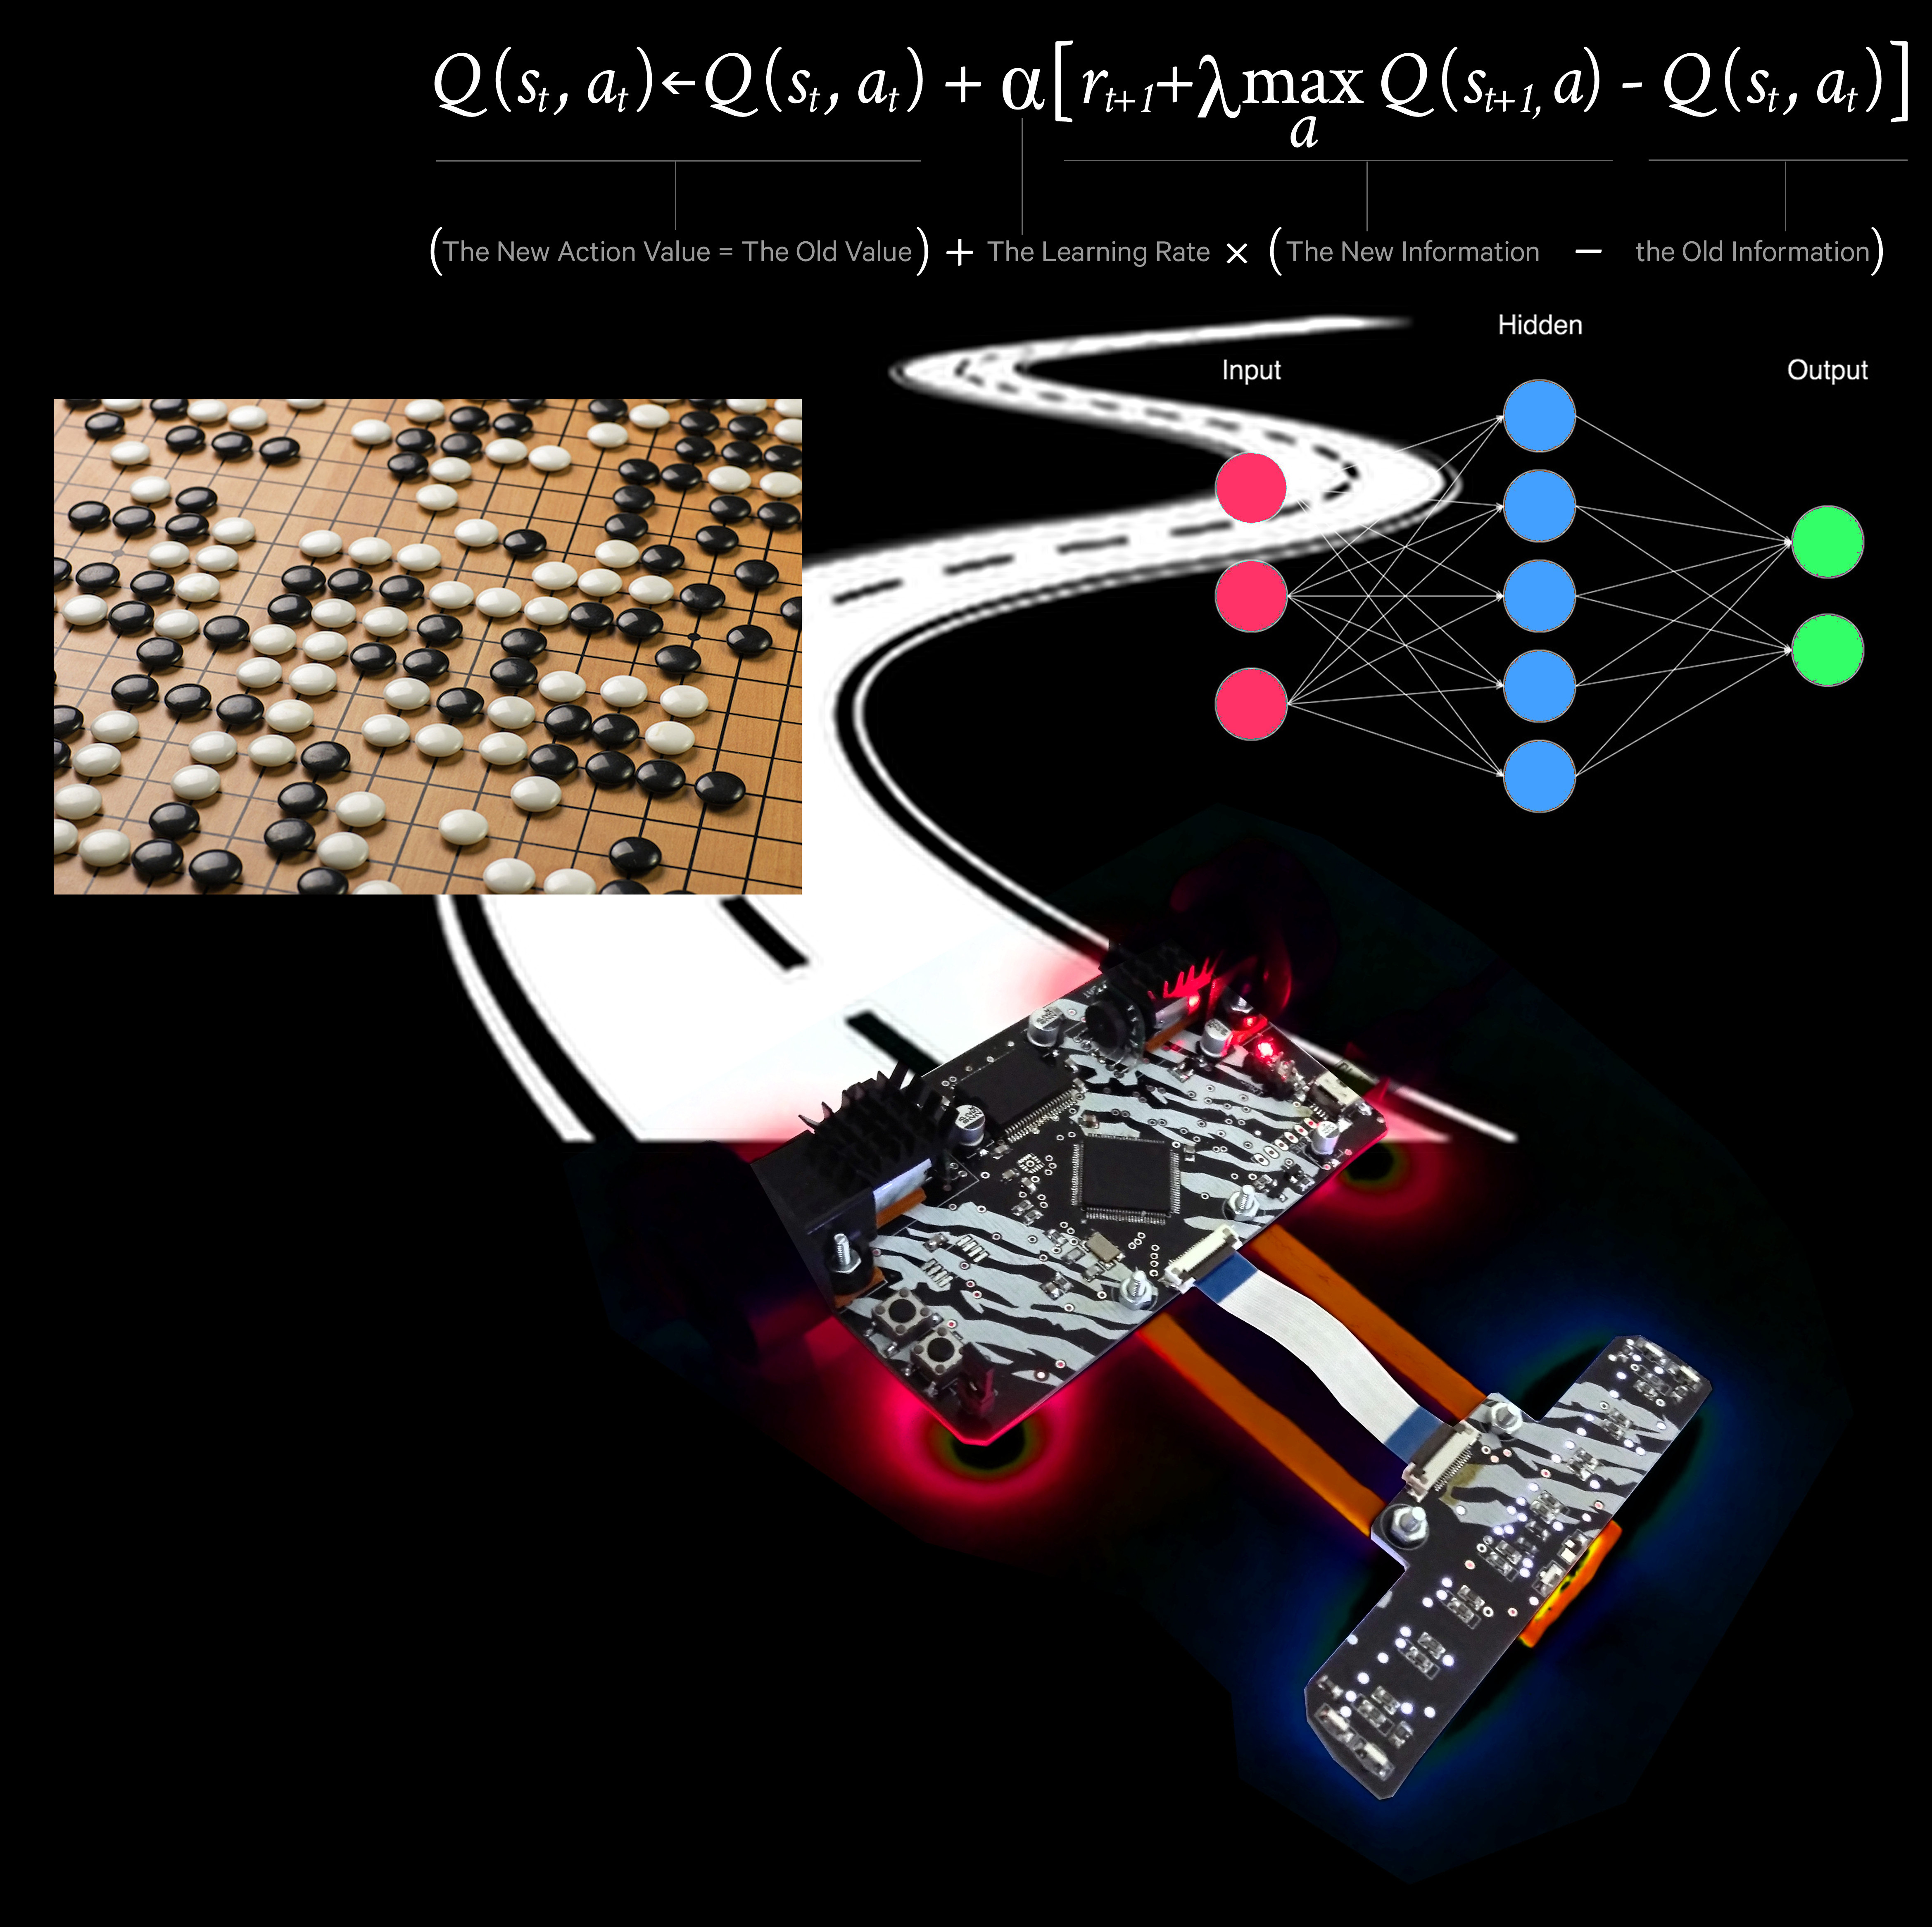
\includegraphics[width=5.05in]{../images/generic/rl_square.jpg}}

        \hfil}\vfil}
    }

    \begin{frame}
     \centering
     \colorbox{black}
     {
        \begin{minipage}{8cm}
           {\LARGE \color{white}{\bf Algorithms for robotics}} \\
           {\LARGE \color{white}{\bf Michal CHOVANEC, PhD.}} \\
       \end{minipage}
     }

    \end{frame}
}




\begin{frame}
  
  \frametitle{\bf motor velocity controller}

  \centering{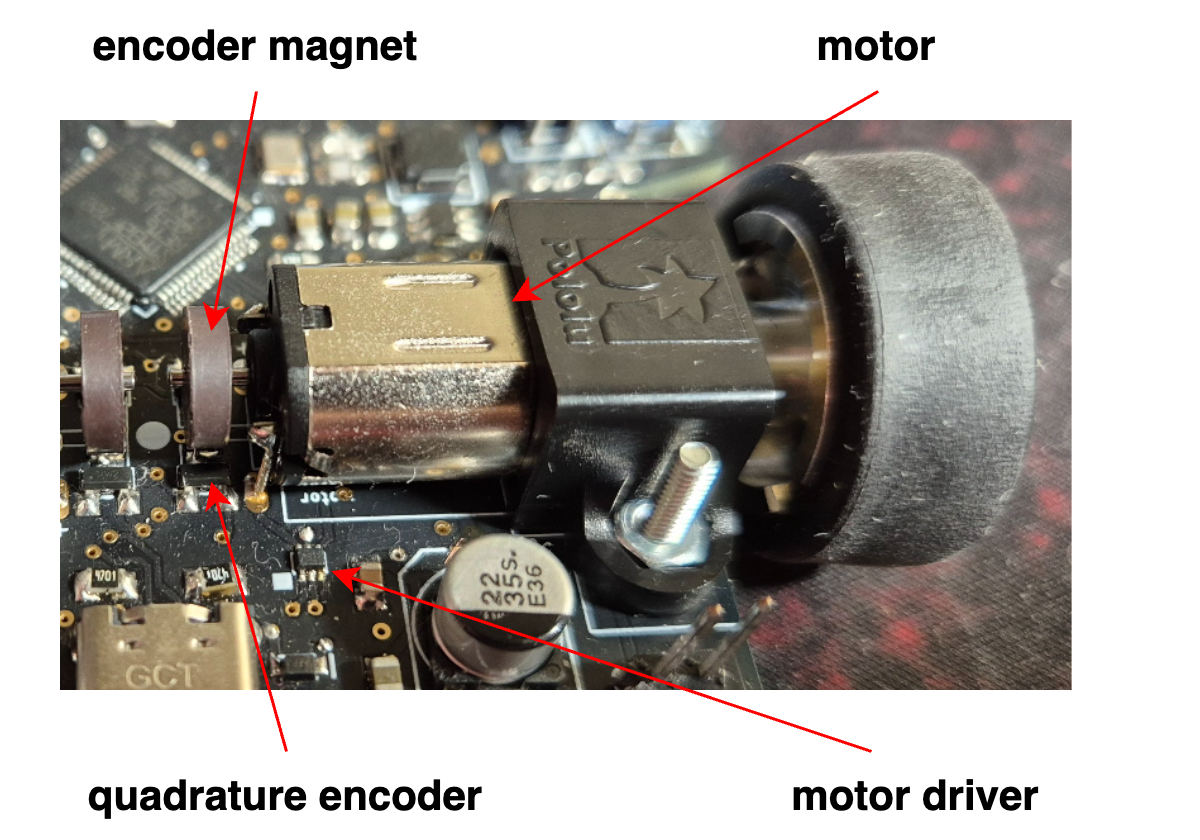
\includegraphics[scale=0.6]{../diagrams/control_generic/control_generic-motor_control_photo.png}}
  \centering{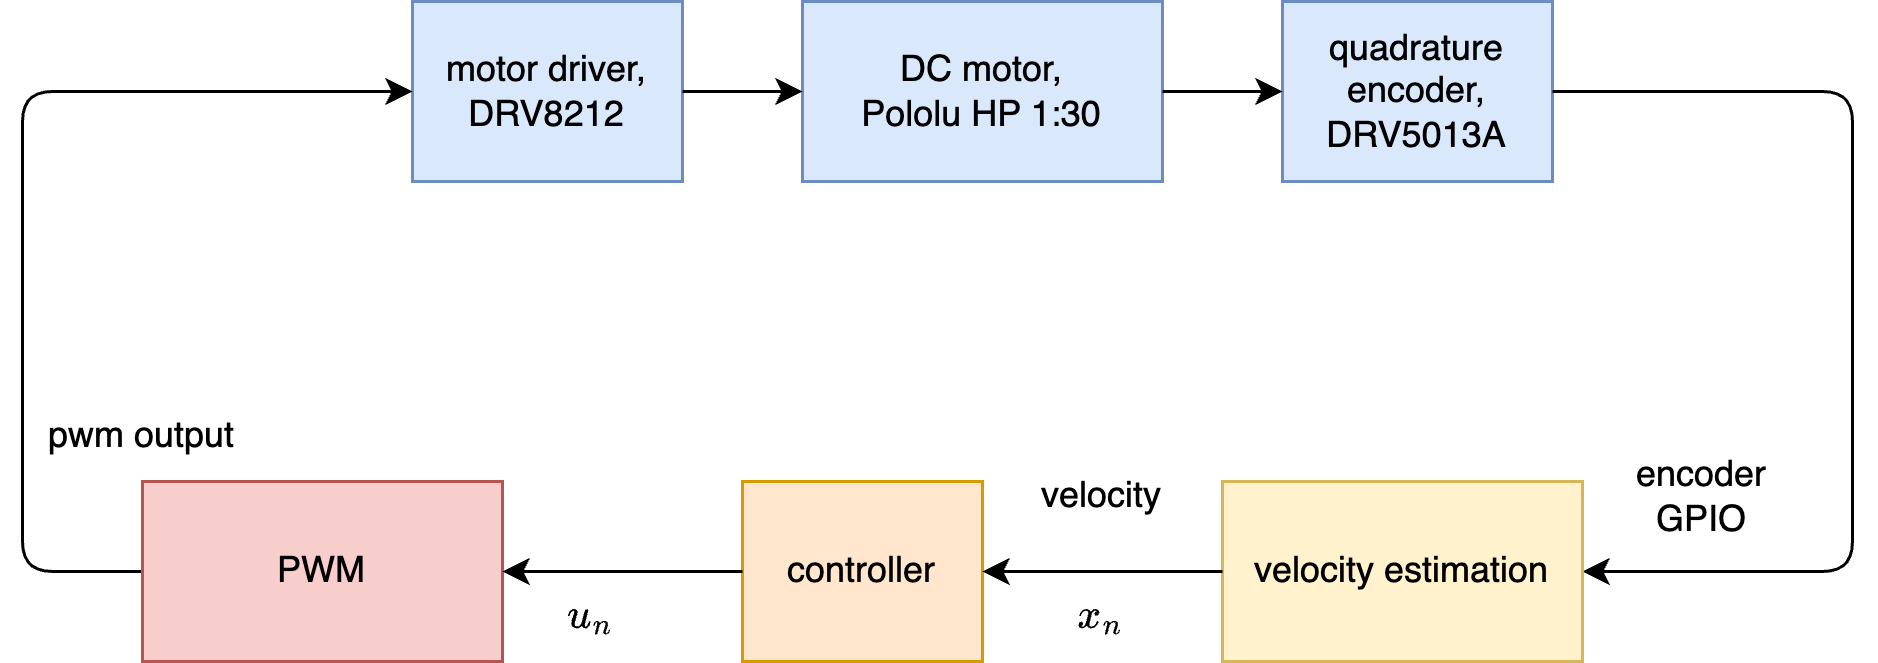
\includegraphics[scale=0.6]{../diagrams/control_generic/control_generic-motor_control.png}}

  
\end{frame}


\begin{frame}
  
  \frametitle{\bf PID control}

  \begin{itemize}
    \item textbook continuous controller 
    {\centering 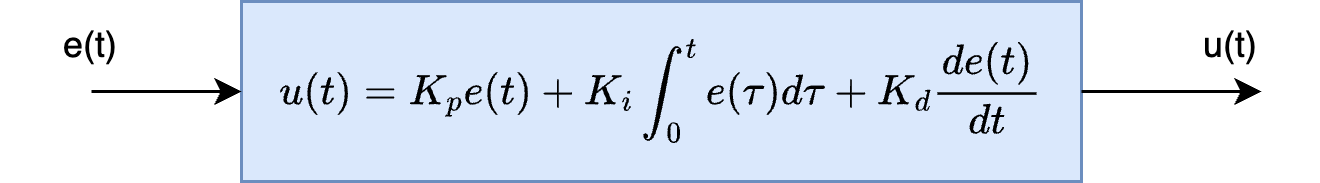
\includegraphics[scale=0.6]{../diagrams/control_generic/control_generic-pid.png}}
    \item discrete controller 
    {\centering 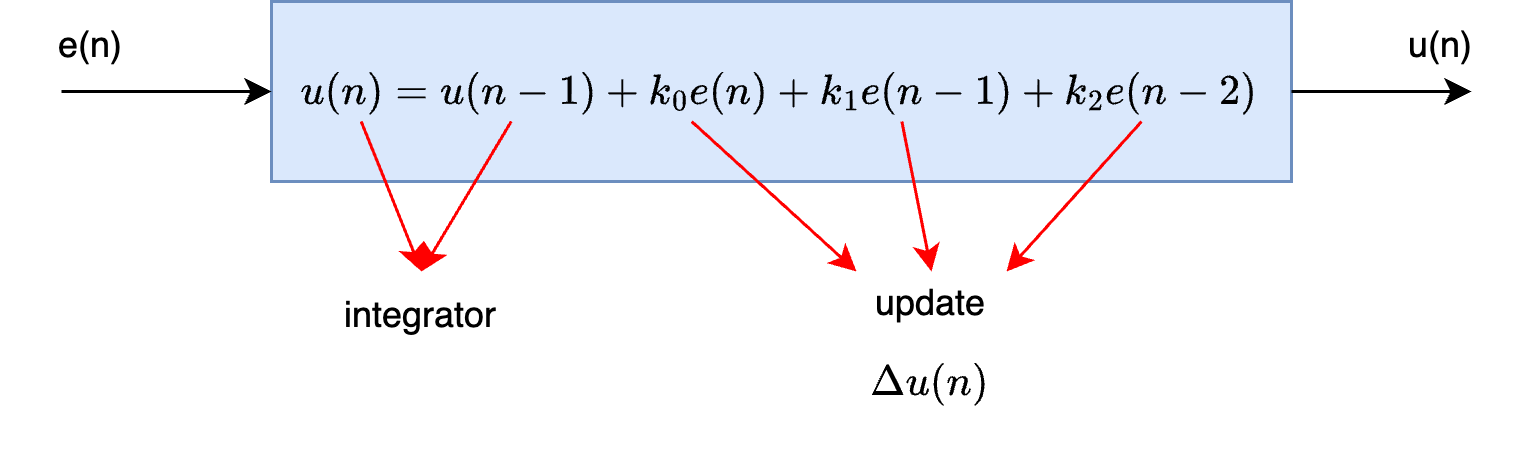
\includegraphics[scale=0.6]{../diagrams/control_generic/control_generic-pid_discrete.png}}
  \end{itemize}

  \begin{align*}
    k_0 &= K_p + K_i\Delta t + \frac{K_d}{\Delta t} \\
    k_1 &= -K_p - 2\frac{K_d}{\Delta t} \\
    k_2 &= \frac{K_d}{\Delta t}
  \end{align*}

\end{frame}



\begin{frame}
  
  \frametitle{\bf PID control - P only}

  \begin{itemize}
    \item  target value : \textcolor{red}{\bf 1000rpm}
    \item  P-only control causes \textcolor{red}{\bf steady state error}
  \end{itemize}
  
 
  \begin{align*}
    u(n+1) &= u(n-1) + k_pe(n) - k_pe(n-1) \\
    k_p    &= 0.01
  \end{align*}

  {\centering 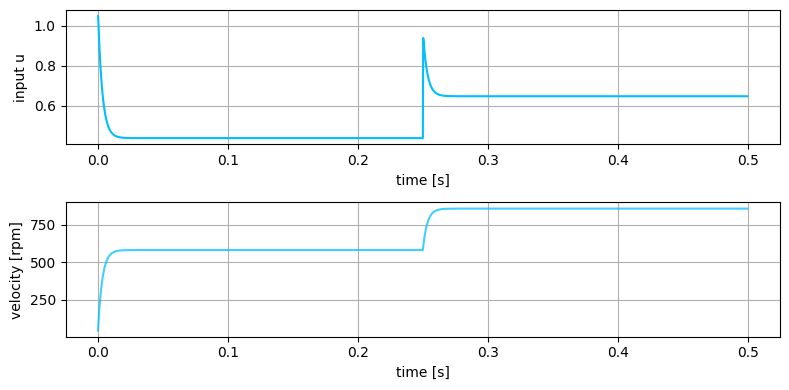
\includegraphics[scale=0.4]{../images/motor_control/pid_p_control.png}}

\end{frame}


\begin{frame}
  
  \frametitle{\bf PID control - PI}

  \begin{itemize}
    \item  target value : \textcolor{red}{\bf 1000rpm}
    \item  PI control \textcolor{red}{\bf removes steady state error}
    \item  too high I term causes \textcolor{red}{\bf oscilations and overshot}
  \end{itemize}

  \begin{align*}
    u(n+1) &= u(n-1) + (k_p + k_i\Delta t) e(n) - k_pe(n-1) \\
    k_p    &= 0.01 \\
    k_i    &= 0.005
  \end{align*}

  {\centering 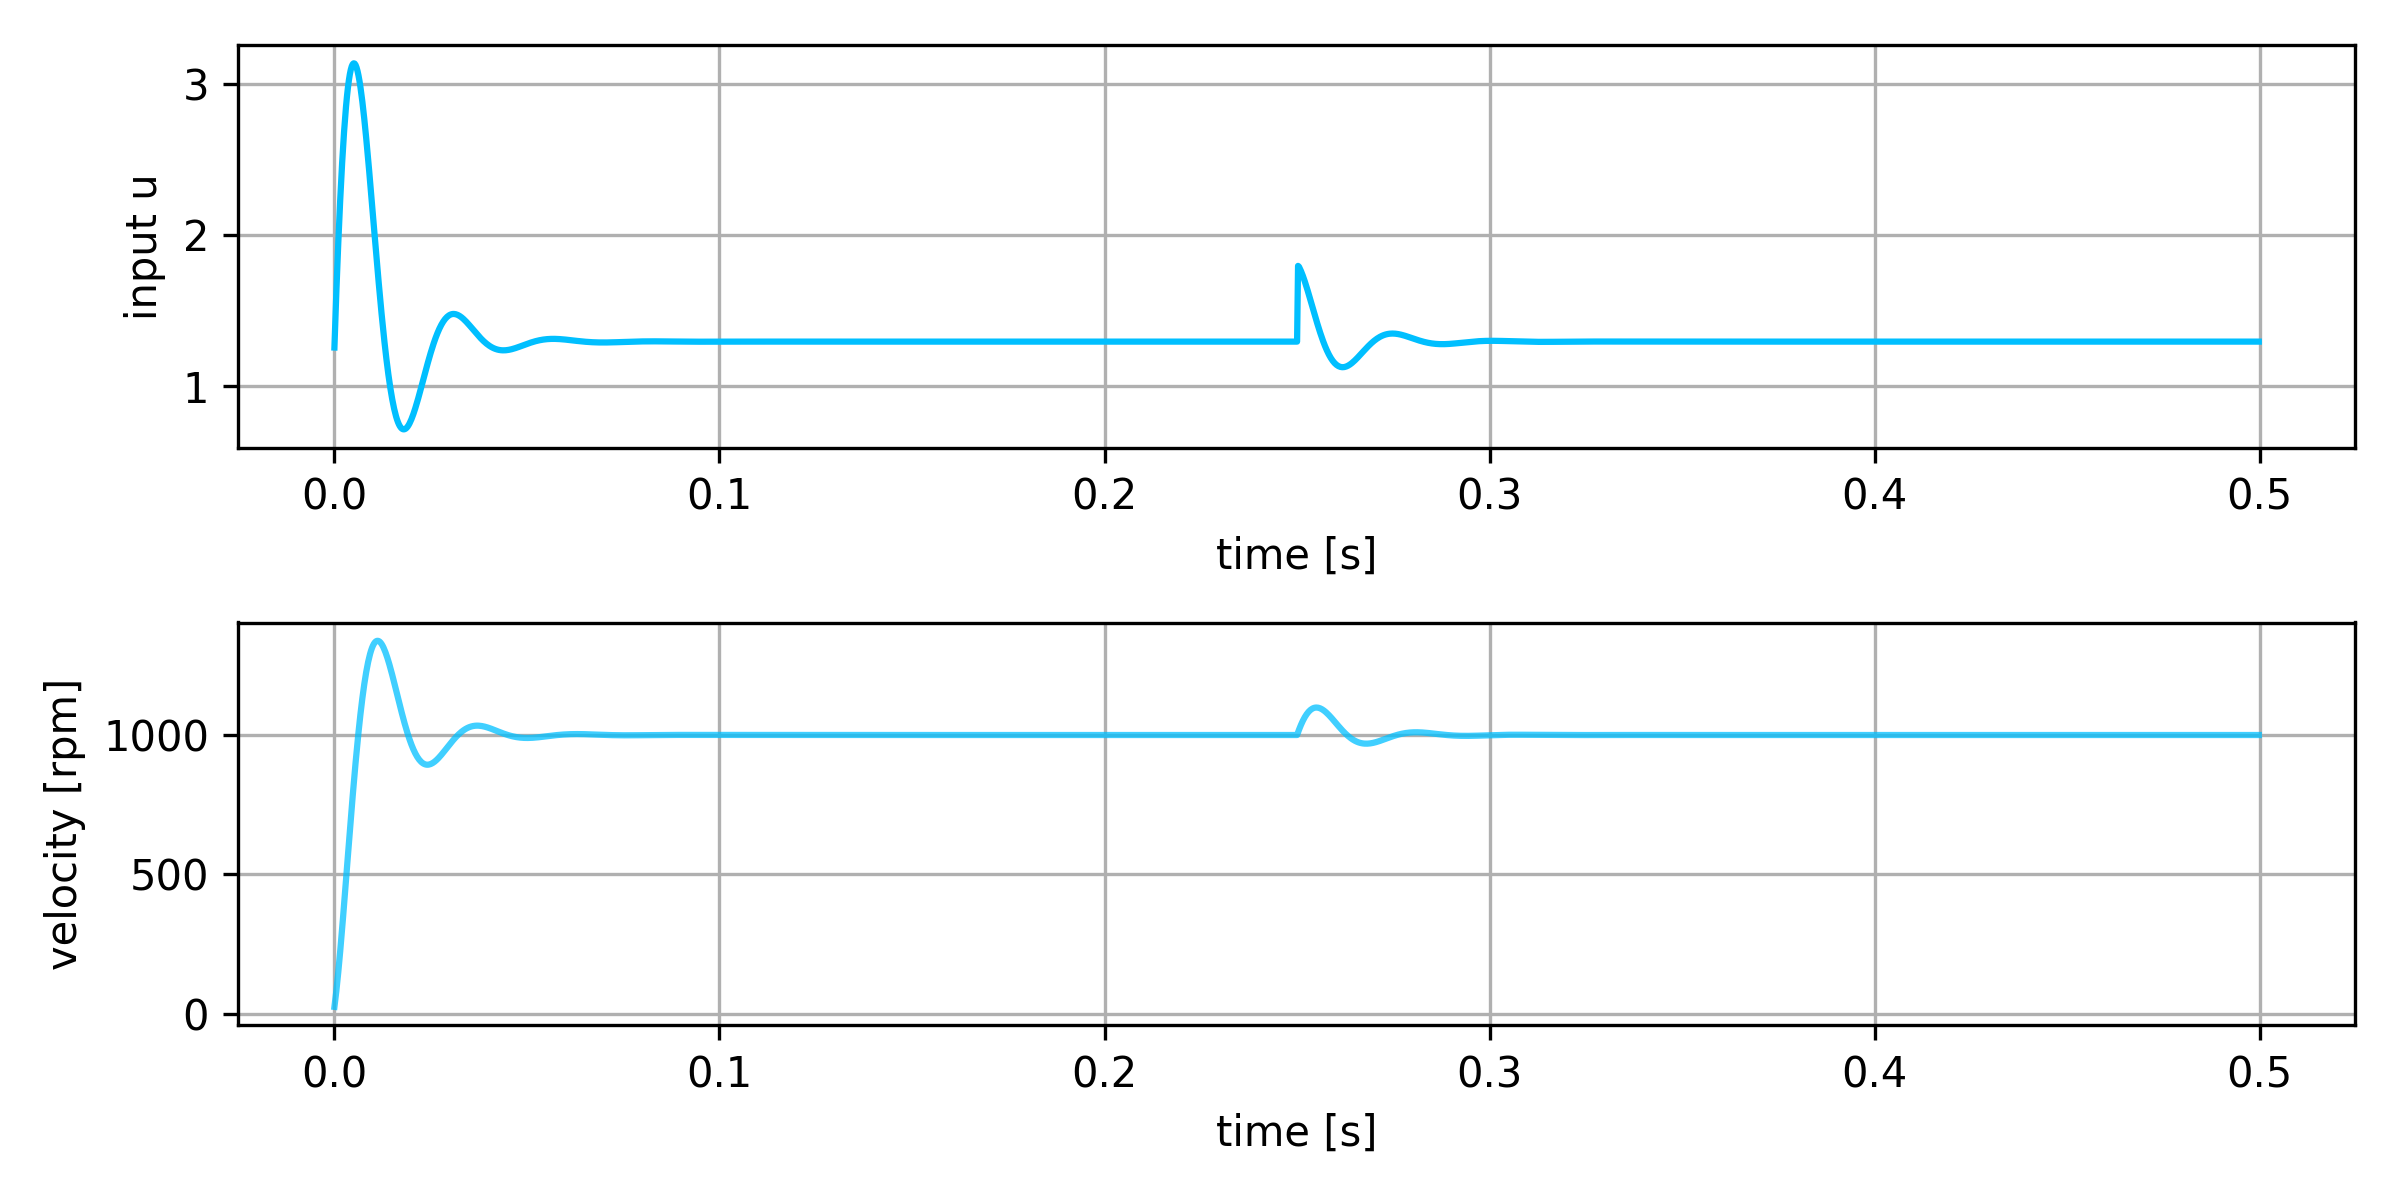
\includegraphics[scale=0.4]{../images/motor_control/pid_pi_control_0.png}}

\end{frame}



\begin{frame}
  
  \frametitle{\bf PID control - PI}

  \begin{itemize}
    \item  target value : \textcolor{red}{\bf 1000rpm}
    \item  correct tunned PI controller for 1st order system
    \item  \textcolor{red}{\bf no overshot, no steady state error}
  \end{itemize}

  \begin{align*}
    u(n+1) &= u(n-1) + (k_p + k_i\Delta t) e(n) - k_pe(n-1) \\
    k_p    &= 0.01 \\
    k_i    &= 0.0002
  \end{align*}

  {\centering 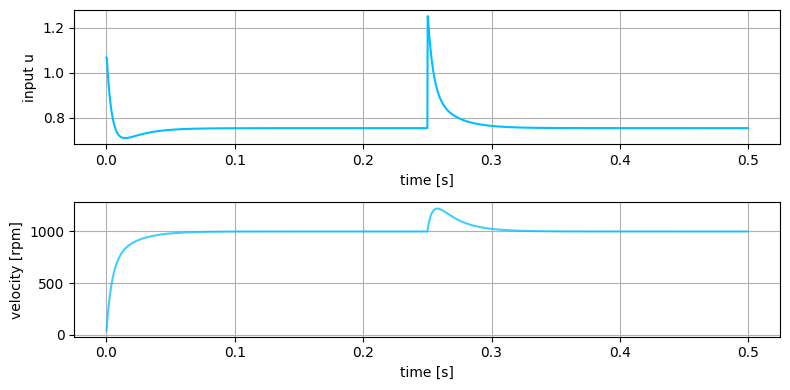
\includegraphics[scale=0.4]{../images/motor_control/pid_pi_control_1.png}}

\end{frame}



\begin{frame}
  
  \frametitle{\bf complete generic discrete PID}

  \begin{enumerate}
    \item  calculate u-change candidate :
      $$\Delta \hat{u}(n) = k_0e(n) + k_1e(n) + k_2e(n)$$
    
    \item clip maximum allowed u-change, to avoid u-kick :
      $$\Delta u(n) = clip(\Delta \hat{u}(n), -du_{min}, du_{max})$$

    \item clip maximum allowed u value, to avoid saturation / windup :
      $$u(n) = clip(u(n-1) + \Delta u(n), -u_{min}, u_{max})$$
  \end{enumerate}
  
\end{frame}



\begin{frame}
  
  \frametitle{\bf complete generic discrete PID}

  {\centering 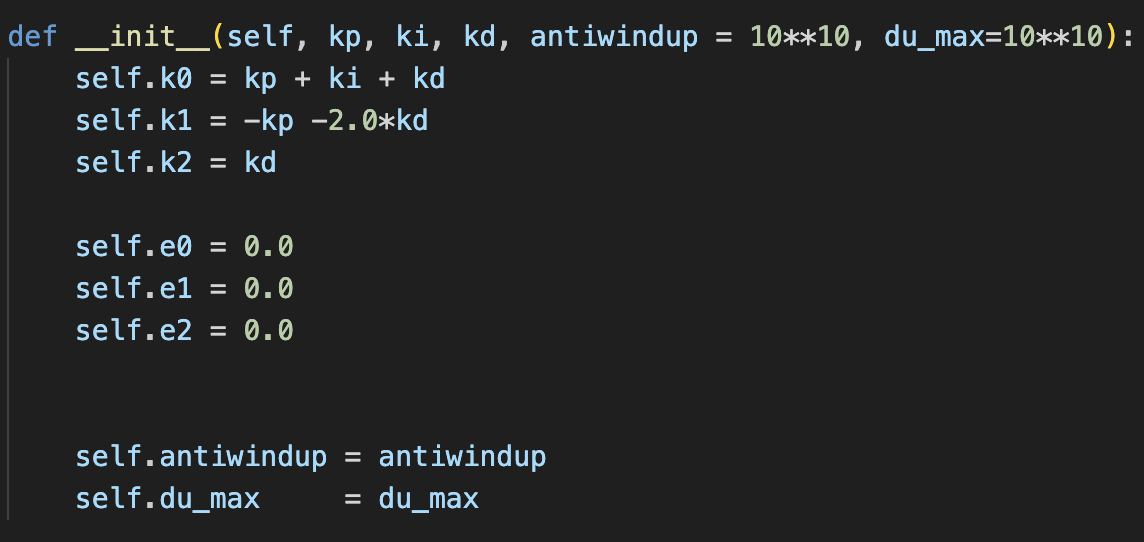
\includegraphics[scale=0.4]{../images/control/pid_init.png}}

  {\centering 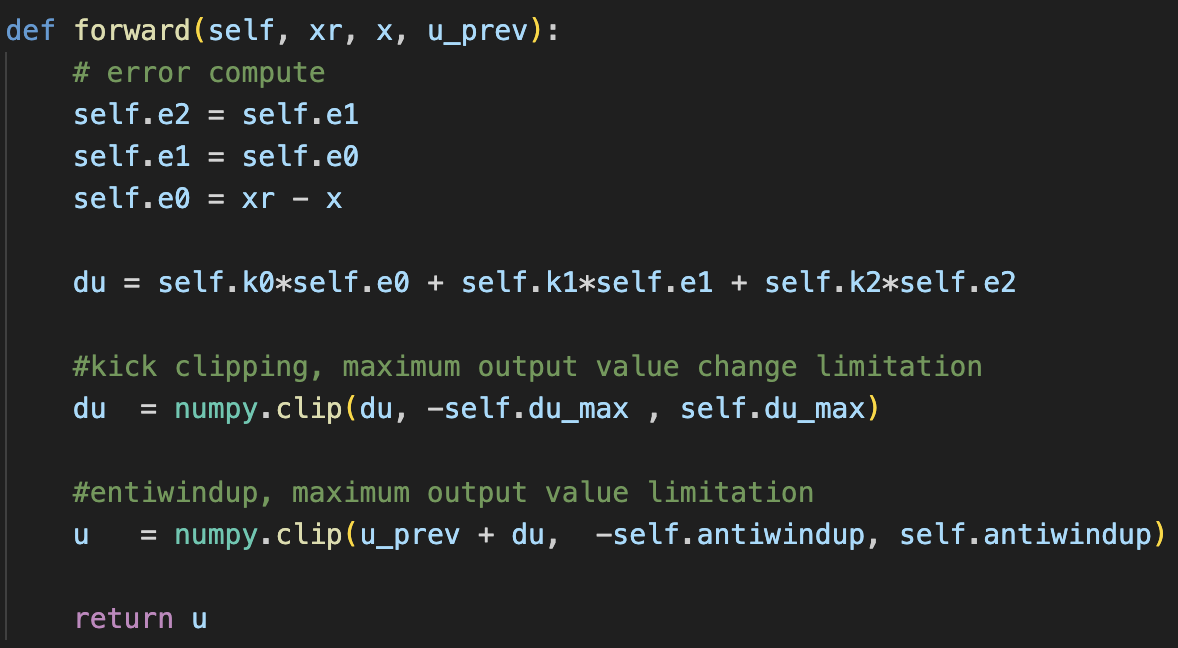
\includegraphics[scale=0.4]{../images/control/pid_main.png}}

  
\end{frame}



\begin{frame}
  
  \frametitle{\bf PID control - issues}

  \begin{itemize}
    \item mostly hand tuned parameters
    \item only single input, single output systems
    \item no implicit noise filtering
  \end{itemize}


\end{frame}




\begin{frame}
  
  \frametitle{\bf motor velocity controller}
  
  \begin{columns}

    \begin{column}{0.5\textwidth}
      \centering{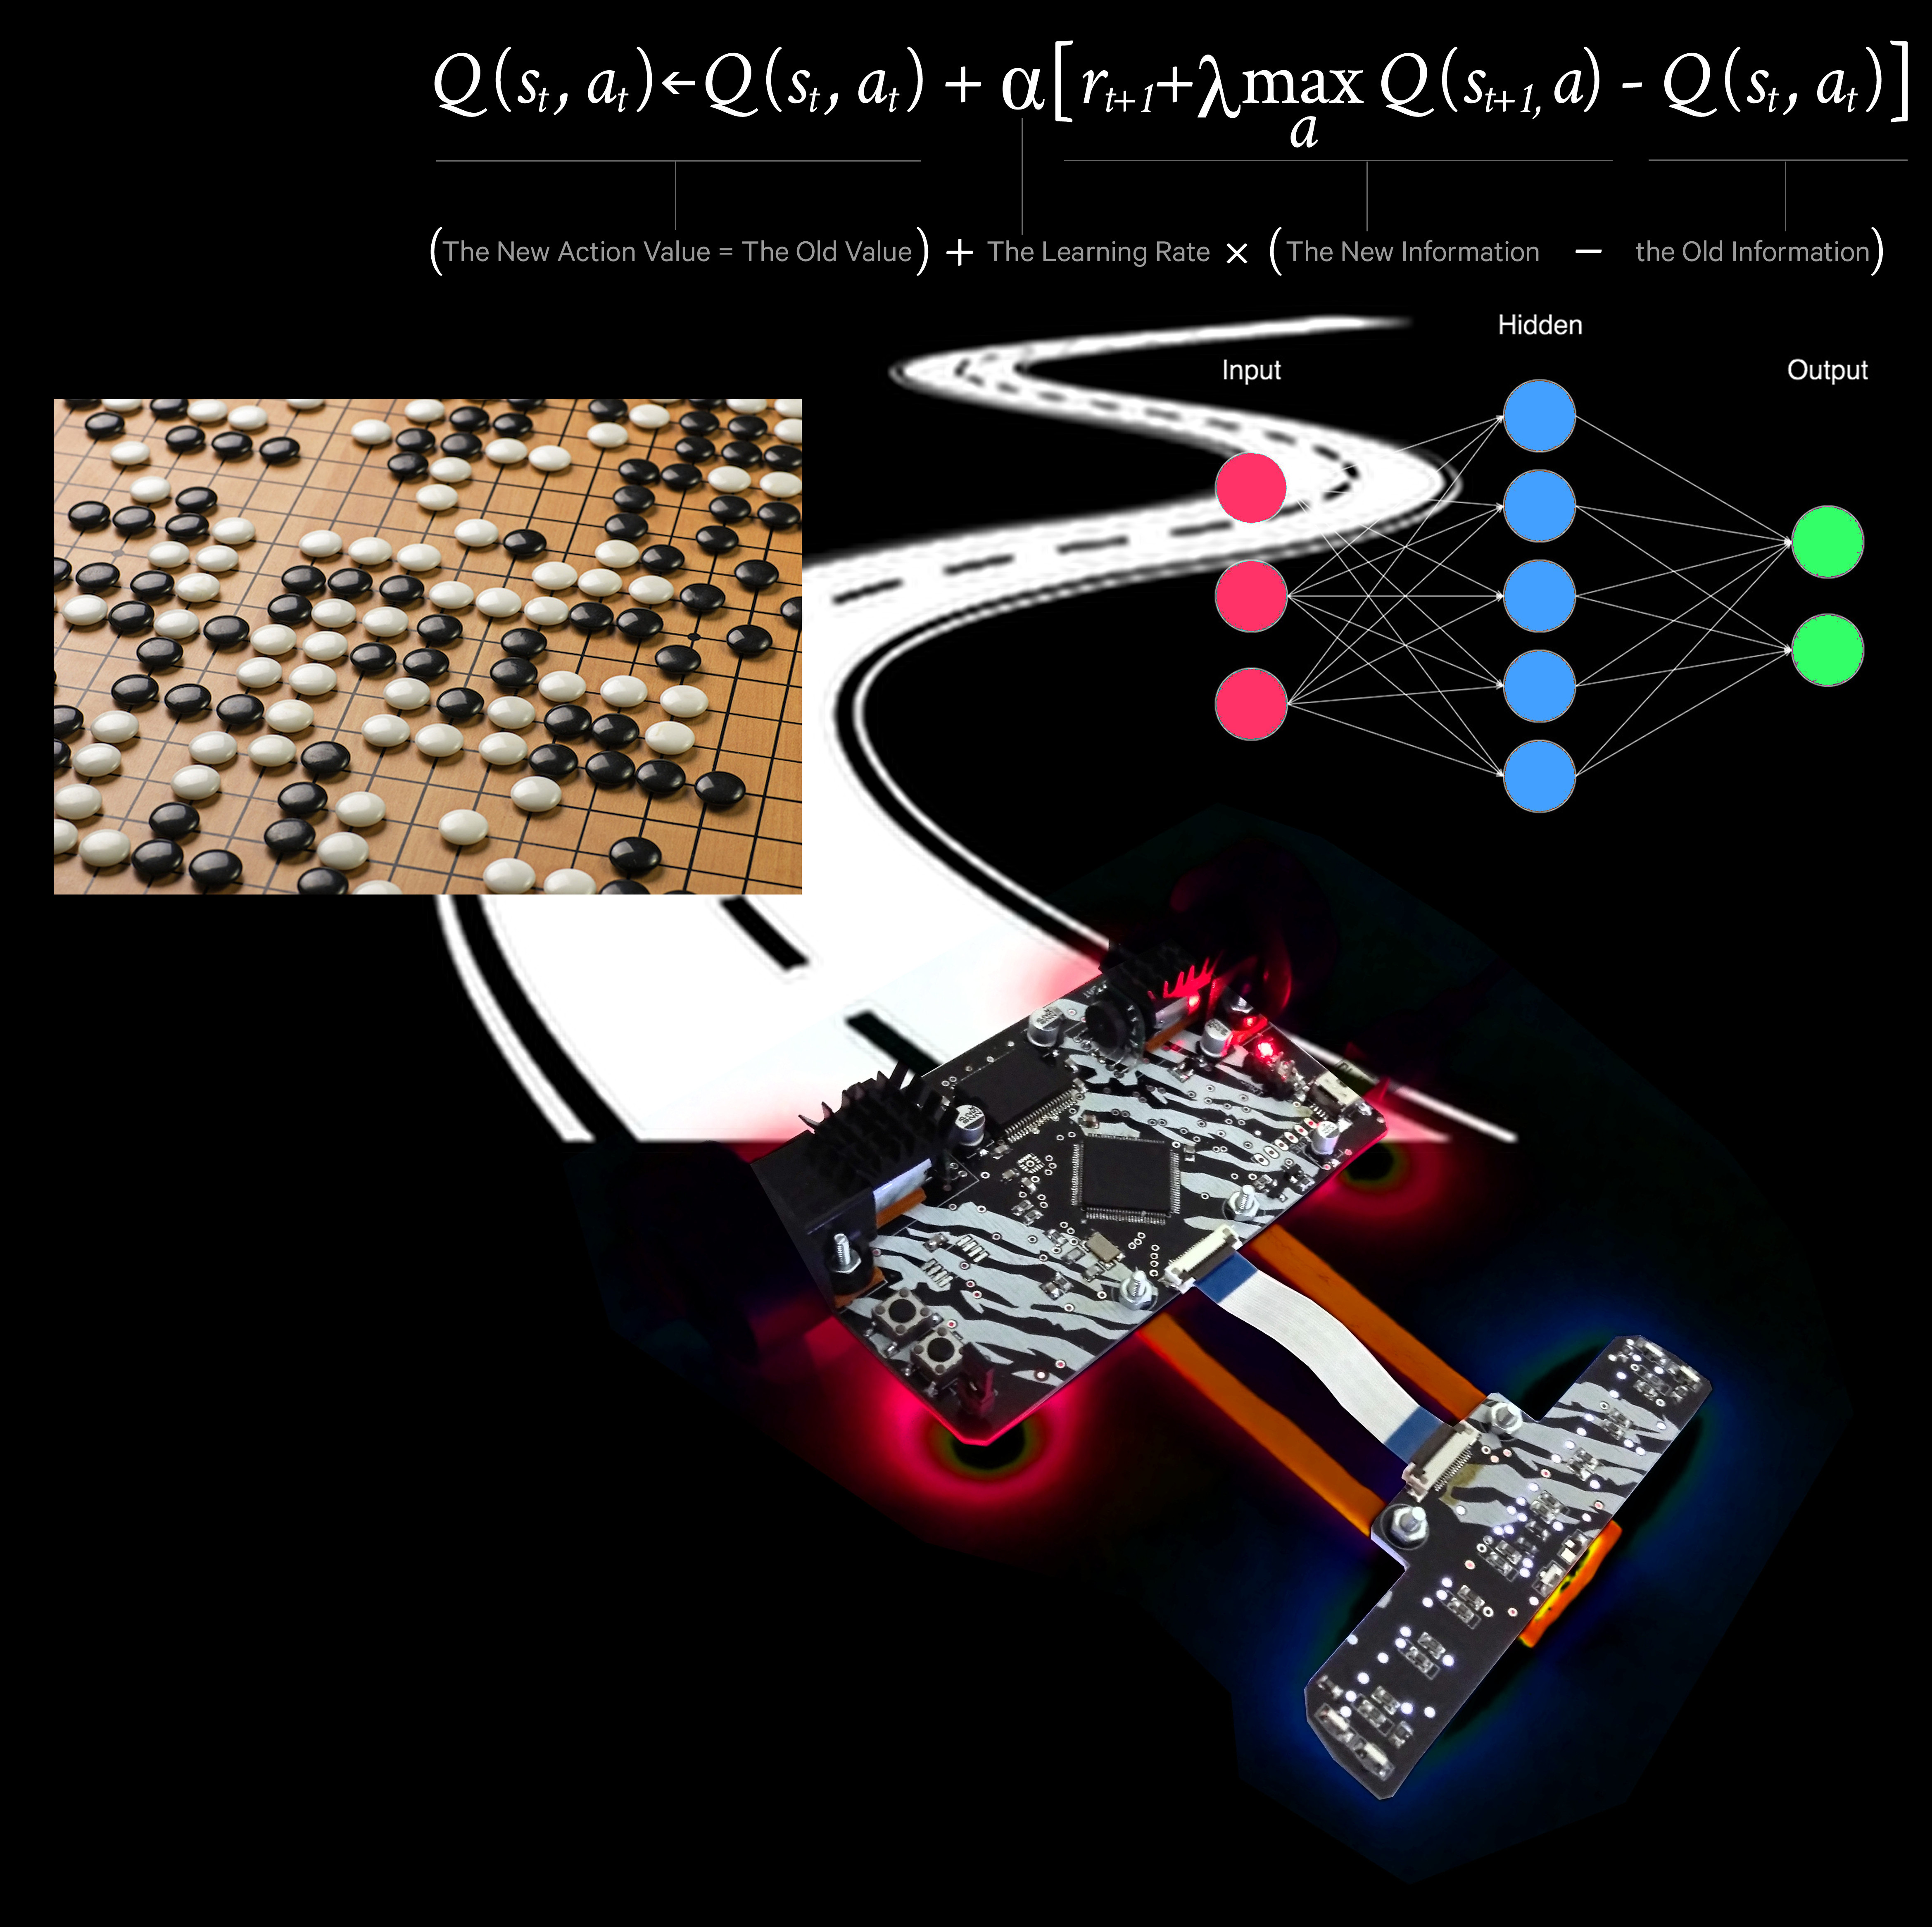
\includegraphics[scale=0.045]{../images/generic/rl_square.jpg}}
    \end{column}

    \begin{column}{0.5\textwidth}
      \begin{itemize}
        \item fastest line following
        \item 3 rounds
        \item obstacles : broken line, brick, loop, colored line
      \end{itemize}
    \end{column}

  \end{columns}
  
\end{frame}


\end{document}